\noindent
\textbf{CHEM 352:
\ifthenelse{\equal{\solutions}{true}}{Examples}{Homework} for chapter 2.}\\

\begin{enumerate}

% Problem 1

\item The quantum mechanical state of a hydrogen atom is described by the following superposition:
$$\psi = \frac{1}{\sqrt{14}}\left(2\psi_{1,0,0} - 3\psi_{2,0,0} - \psi_{3,2,2}\right)$$

where $\psi_{n,l,m}$ are eigenfunctions of the Hamiltonian. The subscripts refer to quantum numbers $n,l,m$.

\begin{enumerate}
\item What is the probability of finding the hydrogen atom in states $(n = 1, l = 0, m = 0), (n = 2, l = 0, m = 0), (n = 3, l = 2, m = 2)$ or in some other state?
\item What are the expectation values for energy, $\vec{\hat{L}}^2$ and $\hat{L}_z$?
\end{enumerate}

\ifthenelse{\equal{\solutions}{true}}{% Problem 1/2 solution
\noindent
\underline{Solution:}\\

First we check that the wavefunctions are normalized. For hydrogenlike atom orbitals we have the following orthonormality condition: $\left<\psi_{n,l,m}\left|\psi_{n',l',m'}\right.\right> = \delta_{nn'}\delta_{ll'}\delta_{mm'}$. The normalization of the given wavefunction can now be evaluated:
\begin{eqnarray}
\nonumber
& & \left<\psi\left|\psi\right.\right> = \frac{1}{14}\left<2\psi_{1,0,0} - 3\psi_{2,0,0} - \psi_{3,2,2}\left|2\psi_{1,0,0} - 3\psi_{2,0,0} - \psi_{3,2,2}\right.\right>\\
\nonumber
& & = \frac{1}{14}(4 + 9 + 1) = 1\textnormal{ (due to orthonormality)}
\end{eqnarray}

\begin{enumerate}
\item The probabilities for the energy eigenstates are given by squaring their coefficients in the wavefunction. The probabilities are then: $P(1,0,0) = 4/14 = 2 / 7, P(2,0,0) = 9/14$ and $P(3,2,2) = 1/ 14$.
\item The expectation value for energy is:
\begin{eqnarray}
\nonumber
& & \left<\psi\left|\hat{H}\right|\psi\right> = \frac{1}{14}\left<2\psi_{1,0,0} - 3\psi_{2,0,0} - \psi_{3,2,2}\left|\hat{H}\right|2\psi_{1,0,0} - 3\psi_{2,0,0} - \psi_{3,2,2}\right>\\
\nonumber
& & = \frac{1}{14}\left(4\overbrace{\left<\psi_{1,0,0}\left|\hat{H}\right|\psi_{1,0,0}\right>}^{=E_{1,0,0}} + 9\overbrace{\left<\psi_{2,0,0}\left|\hat{H}\right|\psi_{2,0,0}\right>}^{= E_{2,0,0}} + \overbrace{\left<\psi_{3,2,2}\left|\hat{H}\right|\psi_{3,2,2}\right>}^{=E_{3,2,2}}\right)\\
\nonumber
& & = \frac{2}{7}E_{1,0,0} + \frac{9}{14}E_{2,0,0} + \frac{1}{14}E_{3,2,2}
\end{eqnarray}

The numerical values for $E_{n,l,m}$'s can be calculated from:
$$E_n = -\frac{hcR}{n^2} = \frac{-13.6\textnormal{ eV}}{n^2} = \frac{E_1}{n^2}$$

Thus the numerical value for $\left<\hat{H}\right>$ is:
$$\left<\hat{H}\right> = \left(\frac{2}{7} + \frac{9}{14}\times\frac{1}{4} + \frac{1}{14}\times\frac{1}{9}\right)E_1 = \frac{229}{504}E_1\approx -6.2\textnormal{ eV}$$

The expectation value for $\vec{\hat{L}}^2$ is:
\begin{eqnarray}
\nonumber
& & \vec{\hat{L}}^2\left|\psi_{n,l,m}\right> = l(l + 1)\hbar^2\left|\psi_{n,l,m}\right>\\
\nonumber
& & \left<\vec{\hat{L}}^2\right> = \frac{\hbar^2}{14}\left(0 + 0 + 2(2 + 1))\right) = \frac{3}{7}\hbar^2
\end{eqnarray}

The expectation value for $\hat{L}_z$ is:
\begin{eqnarray}
\nonumber
& & \hat{L}_z\left|\psi_{n,l,m}\right> = m\hbar\left|\psi_{n,l,m}\right>\\
\nonumber
& & \left<\hat{L}_z\right> = \frac{\hbar}{14}(0 + 0 + 2) = \frac{1}{7}\hbar
\end{eqnarray}

\end{enumerate}

\hrule\vspace{0.5cm}
}{}

% Problem 2

\item Show that operators $\hat{L}_z$ and $\vec{\hat{L}}^2 = \hat{L}_x^2 + \hat{L}_y^2 + \hat{L}_z^2$ commute with the hydrogen atom Hamiltonian operator:
$$\left[-\frac{\hbar^2}{2m}\Delta + \hat{V}, \hat{L}_z\right] = \left[-\frac{\hbar^2}{2m}\Delta + \hat{V}, \vec{\hat{L}}^2\right] = 0$$

where $\hat{V}$ is the operator corresponding to electron - nuclear Coulomb interaction. Use spherical coordinates and remember that operators commute, for example, if they depend on different variables. What is the significance of this result?

\ifthenelse{\equal{\solutions}{true}}{% Problem 2/2 solution
\noindent
\underline{Solution:}\\

The Hamiltonian consists of the kinetic energy part, which is proportional to the Laplacian operator, and the Coulomb potential.
Laplacian in spherical coordinates is (see lecture notes or a tablebook):

$$\Delta\equiv \nabla^2 = \frac{1}{r^2}\frac{\partial}{\partial r}\left(r^2\frac{\partial}{\partial r}\right) + \frac{1}{r^2\sin(\theta)}\frac{\partial}{\partial\theta}\left(\sin(\theta)\frac{\partial}{\partial\theta}\right)
+ \frac{1}{r^2\sin^2(\theta)}\frac{\partial^2}{\partial\phi^2}$$

The Coulomb potential depends on only on spatial coordinate $r$ (e.g. the distance between the nucleus and the electron). The $\hat{L}_z$ operator is defined in spherical coordinates as:

$$\hat{L}_z = -i\hbar\frac{\partial}{\partial\phi}$$

This clearly commutes with the first two terms in the Laplacian because those terms do not depend on $\phi$. The third depends on $\phi$ but both operators consist of differentiation with respect to $\phi$ and hence they commute. Thus $\left[\hat{H},\hat{L}_z\right] = 0$.

Next we consider $\vec{\hat{L}}^2$. This is operator can be written in spherical coordinates as:
$$\vec{\hat{L}}^2 = -\hbar^2\left[\frac{1}{\sin(\theta)}\frac{\partial}{\partial\theta}\left(\sin(\theta)\frac{\partial}{\partial\theta}\right) + \frac{1}{\sin^2(\theta)}\frac{\partial^2}{\partial\phi^2}\right]$$

This does not depend on $r$ and therefore it commutes with the Coulomb potential and the first term in the Laplacian, which depends only on $r$. Apart from $r$ and some constants $\vec{\hat{L}}^2$ is identical to the angular part of the Laplacian. Operators always commute with themselves. Thus $\left[\hat{H},\vec{\hat{L}}^2\right]$. The significance of these results is that both the energy and the quantum numbers $l$ and $m_l$ can be specified simultaneously.

\hrule\vspace{0.5cm}
}{}

% Problem 3

\item Demonstrate that the Cartesian hydrogen like $p_x$ and $p_y$ orbitals are not eigenfunctions of $\hat{L}_z$ but their linear combinations $p_x \pm ip_y$ are.

\ifthenelse{\equal{\solutions}{true}}{% Problem 3/2 solution
\noindent
\underline{Solution:}\\

$$M = y^2 -xy\textnormal{ and }N = -x^2$$

$$\left(\frac{\partial M}{\partial y}\right)_x = 2y - x\textnormal{ and }\left(\frac{\partial N}{\partial x}\right)_y = -2x$$

Because the partial derivatives are not equal, the differential is inexact. If we divide the differential by $xy^2$, we have:

$$M = \frac{1}{x} - \frac{1}{y}\textnormal{ and }N = -\frac{x}{y^2}$$

$$\left(\frac{\partial M}{\partial y}\right)_x = \frac{1}{y^2}\textnormal{ and }\left(\frac{\partial N}{\partial x}\right)_y = -\frac{1}{y^2}$$

and hence differential $\frac{df}{xy^2}$ is inexact (difference in sign only!).

\hrule\vspace{0.5cm}
}{}

% Problem 4

\item 

\begin{enumerate}
\item Consider a hydrogenlike atom with on electron on $2s$ orbital. What is the most probable distance from the nucleus? Use the radial wavefunction in your calculation.
\item Show that the following hydrogenlike atom orbital pairs are orthogonal: ($1s,2s$) and ($2p_x, 2p_y$).
\end{enumerate}

\ifthenelse{\equal{\solutions}{true}}{% Problem 4/2 solution
\noindent
\underline{Solution:}\\

\begin{enumerate}

\item \underline{Isothermal process A.} Temperature after A, denoted by $T_2$, is given by the ideal gas law:

$$T_2 = \frac{P_2V_2}{nR} = \frac{(2000\times 10^3\textnormal{ N m}^{-2})(10^{-3}\textnormal{ m}^3)}{(1\textnormal{ mol})(8.314\textnormal{ N m mol}^{-1}\textnormal{ K}^{-1})} = 240.6\textnormal{ K}$$

Both $U$ and $H$ depend only on temperature for ideal gases. This is an isothermal process and hence both $\Delta U$ and $\Delta H$ are zero. The $PV$-work in this step is given by (see lecture notes):

$$w_{rev} = -nRT\ln\left(\frac{V_2}{V_1}\right)$$
$$ = -\left(1\textnormal{ mol}\right)\times\left(8.314\textnormal{ J mol}^{-1}\textnormal{ K}^{-1}\right)\times\left(240.6\textnormal{ K}\right)\times\ln\left(\frac{1\textnormal{ dm}^3}{10\textnormal{ dm}^3}\right) = 4.6\textnormal{ kJ}$$

According to the first law of thermodynamics:

$$\Delta U = q + w \Rightarrow q = \Delta U - w = 0 - 4.6\textnormal{ kJ} = -4.6\textnormal{ kJ}$$

\item \underline{Isobaric process B.} The temperature at 3 is given by the ideal gas law:

$$T_3 = \frac{P_3V_3}{nR} = \frac{(2000\times10^3\textnormal{ N m}^{-2})(10^{-2}\textnormal{ m}^3)}{(1\textnormal{ mol})(8.314\textnormal{ N m mol}^{-1}\textnormal{ K}^{-1})} = 2406\textnormal{ K}$$

Changes in the internal energy and enthalpy are given by:

$$\Delta U = \frac{3}{2}nR\Delta T = \frac{3}{2}nR\left(T_3 - T_2\right)$$
$$ = 1.5 \times (1\textnormal{ mol}) \times\left( 8.314\textnormal{ J mol}^{-1}\textnormal{ K}^{-1}\right) \times \left( 2406\textnormal{ K} - 240.6\textnormal{ K} \right) = 27.0\textnormal{ kJ}$$
$$\Delta H = \frac{5}{2}nR\Delta T = 45.0\textnormal{ kJ}$$

The first law states: $\Delta U = q + w$ and thus if we know either $q$ or $w$, we can always calculate the other. In the isobaric case the work can be obtained with $P_{ext} = P$ and $dw = -P dV$. Integration of this equation gives: $w = -P\Delta V = -(2000 \times 10^3\textnormal{ Nm}^{-2}) \times (10 \times 10^{-3}\textnormal{ m}^3 - 1.0 \times 10^{-3}\textnormal{ m}^3) = -18.0\textnormal{ kJ}$. And further $q = 27.0\textnormal{ kJ} - (-18.0\textnormal{ kJ}) = 45.0\textnormal{ kJ}$.

\item \underline{Isochoric process C.} The temperature at point 1 is given by the ideal gas law:

$$T_1 = \frac{P_1V_1}{nR} = 240.6\textnormal{ K}$$

Changes in the internal energy and enthalpy are given by:

$$\Delta U = \frac{3}{2}nR\Delta T = 1.5\times \left(1\textnormal{ mol}\right) \times \left( 8.314\textnormal{ J mol}^{-1}\textnormal{ K}^{-1}\right)$$
$$\times\left(240.6\textnormal{ K} - 2406\textnormal{ K}\right) = -27.0\textnormal{ kJ}$$

$$\Delta H = \frac{5}{2}nR\Delta T = 2.5\times \left(1\textnormal{ mol}\right) \times \left( 8.314\textnormal{ J mol}^{-1}\textnormal{ K}^{-1}\right)$$
$$\times\left(240.6\textnormal{ K} - 2406\textnormal{ K}\right) = -45.0\textnormal{ kJ}$$

The volume is constant and hence $w = 0$ kJ. The first law gives $q = -27.0$ kJ. The total work in the cycle is: $w_{tot} = w_{\textnormal{A}} + w_{\textnormal{B}} + w_{\textnormal{C}} = (4.61 - 18.0 + 0.00)\textnormal{ kJ} = -13.4\textnormal{ kJ}$.

\end{enumerate}

\hrule\vspace{0.5cm}
}{}

% Problem 5

\item 

\begin{enumerate}
\item Write the electron configuration for V$^{2+}$ ion. What quantum numbers for the total electron spin are possible in this configuration?
\item If two electrons reside on two different orbitals, what are the possible values for total spin and the multiplicity? What values are possible for three electrons on different orbitals?
\end{enumerate}

\ifthenelse{\equal{\solutions}{true}}{% Problem 5/2 solution
\noindent
\underline{Solution:}\\

\begin{itemize}
\item[a)] Based on the lecture notes, we have:

$$w = RT\ln\left(\frac{P_2}{P_1}\right) = \left(8.314\textnormal{ J K}^{-1}\textnormal{ mol}^{-1}\right)\times\left(298.15\textnormal{ K}\right)\times\ln\left(\frac{0.132\textnormal{ bar}}{1\textnormal{ bar}}\right)$$
$$ = -5.03\textnormal{ kJ mol}^{-1}$$

\item[b)] In (a) the pressure changes during the process. Here the external pressure is constant and we can directly calculate:

$$w = -P_{ext}\Delta V = -P_{ext}\left(V_2 - V_1\right)$$
$$V_1 = \frac{nRT}{P_1} = 0.0248\textnormal{ m}^3\textnormal{ and }V_2 = 0.188\textnormal{ m}^3$$

$$\Rightarrow w = -\left(0.132\times 10^5\textnormal{ N m}^{-2}\right)\left(0.188\textnormal{ m}^3 - 0.0248\textnormal{ m}^3\right) = -2.15\textnormal{ kJ mol}^{-1}$$

\end{itemize}

\hrule\vspace{0.5cm}
}{}

% Problem 6

\item 

\begin{enumerate}
\item What information do the following term symbols provide about a given atom: $^1D_2$ and $^3F_4$?
\item Consider the emission spectrum of potassium atom, which exhibits lines at $\lambda_1 = 766.70$ nm and $\lambda_2 = 770.11$ nm. What is the value of the spin-orbit coupling constant? The emission lines originate from the $^2P$ excited state (spin-orbit split).
\item Which of the following atomic transitions are (dipole) allowed: $5d\rightarrow 2s, 5p \rightarrow 3s, 5p \rightarrow 3f$?
\end{enumerate}

\ifthenelse{\equal{\solutions}{true}}{% Problem 6/2 solution
\noindent
\underline{Solution:}\\

\begin{enumerate}
\item In $^1D_2$ state there are no unpaired electrons (singlet state) and hence the total spin $S = 0$. The angular momentum quantum number $L = 2$, which means that the total angular momentum $\left<\vec{\hat{L}}^2\right> = 2(2 + 1)\hbar^2 = 6\hbar^2$. The total angular momentum quantum number $J = 2$ (specified by the subscript). In $^3F_4$ state the multiplicity ($2S+1$) is 3 which gives $S = 1$ (triplet state) and $F$ term implies $L = 3$. The total angular momentum quantum number is specified as $J = 4$.
\item The energy level diagram for alkai metal atoms is:

\begin{figure}[htp!]
\centering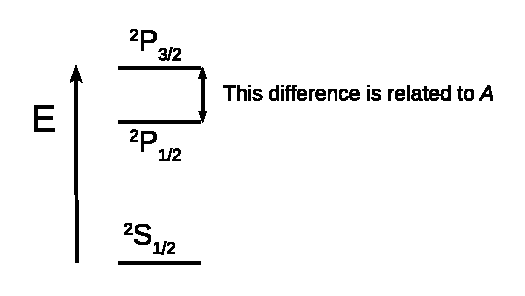
\includegraphics[scale=0.7]{diagram}
\end{figure}

The two emission lines originate from the two $^2P$ states, which are split by the spin-orbit interaction, and terminate to the ground $^2S$ state.
Hence the energy difference between the two emission lines gives the energy difference between the spin-orbit split states $^2P_{1/2}$ and $^2P_{3/2}$.
The line positions must be converted to energy by relation $E = h\nu = \frac{hc}{\lambda}$ ($h$ is the Planck's constant and $c$ is the speed of light).
To calculate $A$, we have to calculate the energy difference between $^2P_{1/2}$ and $^2P_{3/2}$:
\begin{eqnarray}
\nonumber
& & ^2P_{1/2}\textnormal{: }E_{SO} = \frac{A}{2}\left[J(J+1) - L(L+1) - S(S+1)\right] = -A\\
\nonumber
& & ^2P_{3/2}\textnormal{: }E_{SO} = \frac{A}{2}\left[J(J+1) - L(L+1) - S(S+1)\right] = \frac{1}{2}A\\
\nonumber
& & \Delta E_{SO} = \frac{3}{2}A
\end{eqnarray}

Next we calculate the energies for the observed transitions. For $^2P_{3/2}\rightarrow ^2S_{1/2}$ we have:
\begin{eqnarray}
\nonumber
& & E_1 = h\nu_1 = hc / \lambda_1 = (6.6261\times 10^{-34}\textnormal{ Js})\times\frac{2.9979\times 10^8\textnormal{m/s}}{766.70\times 10^{-9}\textnormal{ m}}\\
\nonumber
& &  = 2.5909\times 10^{-19}\textnormal{ J} = 1.6171\textnormal{ eV} = 13043\textnormal{ cm}^{-1}
\end{eqnarray}

For $^2P_{1/2}\rightarrow ^2S_{1/2}$:

\begin{eqnarray}
\nonumber
& & E_2 = h\nu_2 = hc / \lambda_2 = (6.6261\times 10^{-34}\textnormal{ Js})\times\frac{2.9979\times 10^8\textnormal{m/s}}{770.11\times 10^{-9}\textnormal{ m}}\\
\nonumber
& &  = 2.5794\times 10^{-19}\textnormal{ J} = 1.6099\textnormal{ eV} = 12985\textnormal{ cm}^{-1}
\end{eqnarray}

Thus the energy difference is $\Delta E_{SO} = 39$ cm$^{-1}$ which gives $A = 2\Delta E_{SO} / 3 = 39$ cm$^{-1}$.

\item The selection rule is $\Delta l = \pm 1$. For $5d\rightarrow 2s$ we have $\Delta l = -2$ and hence it is forbidden. Transition $5p\rightarrow 3s$ has $\Delta l = -1$ and therefore it is allowed. $5p\rightarrow 3f$ has $\Delta l = +2$ and it is forbidden.

\end{enumerate}

\hrule\vspace{0.5cm}
}{}

% Problem 7

\item

\begin{enumerate}
\item Write all the term symbols that can be obtained from the following electron configurations: $2s^12p^1$, $2p^13d^1$ and Ar$4s^23d^{10}4p^5$ (Br atom).
\item Write the term symbols for carbon atom (He$2d^22p^2$), which has two equivalent $p$-electrons. Hint: tabulate all possible $m_{l_1}, m_{l_2}, m_{s_1}$ and $m_{s_2}$ values and calculate the total $L$ and $S$ values. Remember to exculde the Pauli forbidden states.
\end{enumerate}

\ifthenelse{\equal{\solutions}{true}}{% Problem 7/2 solution
\noindent
\underline{Solution:}\\

\begin{enumerate}
\item Consider $2s^12p^1$ electron configuration. The $s$-shell has $l_1 = 0$ with $s_1 = 1/2$ and $p$-shell has $l_2 = 1$ and $s_2 = 1/2$.
The total $L = l_1 + l_2, ..., \left|l_1 - l_2\right| = 1$. The total spin $S = s_1 + s_2, ..., \left|s_1 - s_2\right| = 1, 0$. Thus the total $J = L + S, ..., \left|L - S\right|$ can be 2, 1 or 0 (for $L = 1, S = 1$) or 1 ($L = 1, S = 0$). This results in the following term symbols: $^3P_2, ^3P_1, ^3P_0$ and $^1P_1$.

For $2p^13d^1$ we can have the following:

$p$-electron: $l_1 = 1, s_1 = 1/2$.\\
$d$-electron: $l_2 = 2, s_2 = 1/2$.\\

Hence $L = 3,2,1$ and $S = 1,0$. This gives the following total $J$ values:

\begin{itemize}
\item $L = 3$ and $S = 1$ results in $J = 4,3,2$ ($^3F_4$, $^3F_3$ and $^3F_2$ term symbols)
\item $L = 3$ and $S = 0$ results in $J = 3$ ($^1F_3$ term symbol)
\item $L = 2$ and $S = 1$ results in $J = 3,2,1$ ($^3D_3$, $^3D_2$ and $^3D_1$ term symbols)
\item $L = 2$ and $S = 0$ results in $J = 2$ ($^1D_2$ term symbol)
\item $L = 1$ and $S = 1$ results in $J = 2,1,0$ ($^3P_2$, $^3P_1$ and $^3P_0$ term symbols)
\item $L = 1$ and $S = 0$ results in $J = 1$ ($^1P_1$ term symbol)
\end{itemize}

For Ar$4s^23d^{10}4p^5$ we have only one unpaired electron which has $l = 1$ and $s = 1/2$. This gives obviously $L = 1$ and $S = 1/2$ and the
total $J = 3/2$ or $1/2$. Hence the two possible term symbols are $^2P_{3/2}$ and $^2P_{1/2}$.

% TODO: Prepare the table...
\item Carbon has 2 equivalent $p$-electrons: $l_1 = l_2 = 1$ and $s_1 = s_2 = 1/2$. We should tabulate all the possible states - including $M_L = m_{l_1} + m_{l_2}$ and $M_S = m_{s_1} + m_{s_2}$.

\end{enumerate}

\hrule\vspace{0.5cm}
}{}

\end{enumerate}
